% ===================================================================
\chapter{Results}
\label{ch:results}

This chapter follows the two stages of Section~\ref{sec:stages}. It first
reports the screening of all eight methods, then breaks down the compression of
the two selected algorithms, and then reports their verification and their
measured performance on the FPGA board. It closes with the two algorithms side
by side.

% -------------------------------------------------------------------
\section{Stage 1: screening eight methods}
\label{sec:stage1}

All eight methods were run over the same 50 consecutive ColoRadar frames, with
all 16 receive channels and \num{9934} reference detections.
Table~\ref{tab:stage1} and Figure~\ref{fig:stage1} give the result.

\begin{table}[htbp]
\centering
\caption[Stage 1: the eight methods]{Stage 1: all eight methods, 50-frame
average, 16 receive channels. ``Missed'' is the false negative rate and FDR the
false discovery rate (Section~\ref{sec:metrics}); NF is the noise floor. DRHE
and LPC predict at lag $\nTx$ and use the original dictionary.}
\label{tab:stage1}
\small
\begin{tabular}{@{}llrrrrr@{}}
\toprule
Method & Type & CR & Missed (\%) & FDR (\%) & NF (dBFS) & SNR (dB)\\
\midrule
FP16       & reference & 1.00 & 0.00  & 0.00 & $-105.64$ & 35.50\\
FX16       & reference & 1.00 & 3.77  & 1.11 & $-105.37$ & 35.36\\
BAQ        & lossy     & 3.76 & 10.44 & 9.69 & $-105.08$ & 35.08\\
RDVLE      & lossy     & 1.12 & 24.01 & 4.62 & $-102.27$ & 33.17\\
RDVLE+UDRE & lossy     & 2.56 & 28.73 & 4.44 & $-101.78$ & 33.00\\
DRHE fp16  & lossless\textsuperscript{*} & 1.04 & 0.05 & 0.01 & $-105.64$ & 35.51\\
\textbf{DRHE} & lossless & \textbf{3.75} & 3.77 & 1.11 & $-105.37$ & 35.36\\
\textbf{LPC}  & lossless & \textbf{3.70} & 3.77 & 1.11 & $-105.37$ & 35.36\\
\bottomrule
\multicolumn{7}{@{}l}{\footnotesize\textsuperscript{*}lossless with respect to its FP16 input, which is itself rounded from the reference.}
\end{tabular}
\end{table}

\begin{figure}[htbp]
\centering
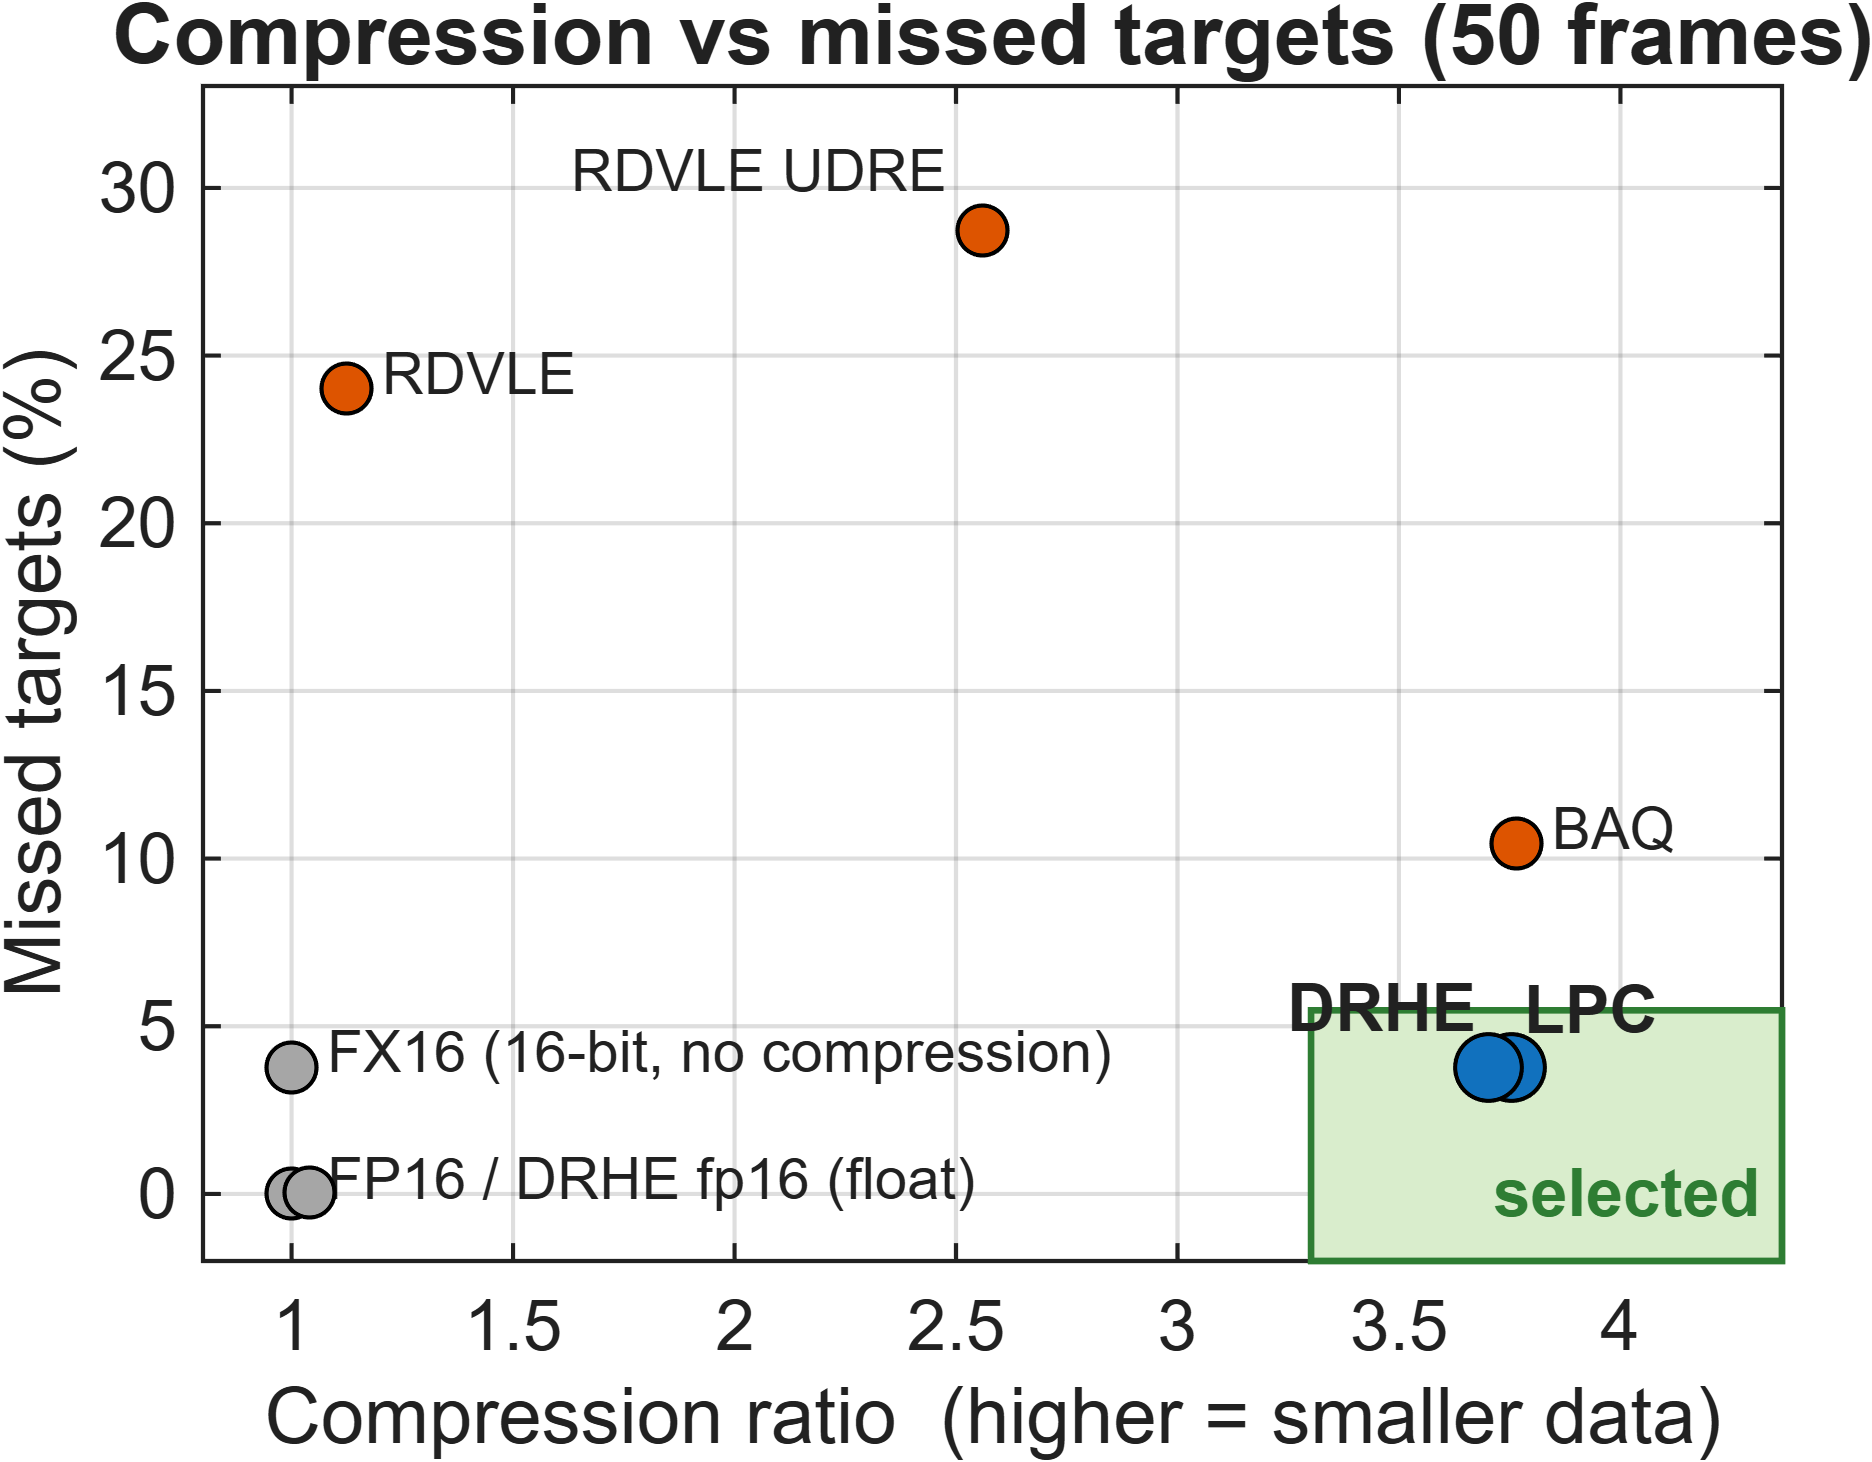
\includegraphics[width=0.62\textwidth]{fig_stage1.png}
\caption[Compression against missed targets]{Compression ratio against missed
targets for the eight methods. A good method sits to the right (small data) and
at the bottom (no extra missed targets). Only DRHE and LPC reach the shaded
region; the lossy methods pay for their ratio in missed targets, and storing
the data as floating point barely compresses.}
\label{fig:stage1}
\end{figure}

Four observations decide what goes forward.

\paragraph{The lossless coders share FX16's detection metrics exactly.}
FX16, DRHE and LPC report identical missed-target rates, false discovery rates,
noise floors and SNR. This is a consequence of losslessness rather than a
coincidence: both coders reconstruct the FX16 codes bit for bit, so the
detector sees identical data. What those rows measure is the cost of the
\emph{quantisation} step, \SI{3.77}{\percent} of targets missed and
\SI{1.11}{\percent} of detections spurious, none of it the cost of compression.

\paragraph{The lossy methods pay for their ratio in detections.}
BAQ reaches \num{3.76}, the same ratio as DRHE, but misses
\SI{10.44}{\percent} of targets instead of \SI{3.77}{\percent}, and
\SI{9.69}{\percent} of what it reports is spurious against
\SI{1.11}{\percent}: nearly three times the miss rate and nearly nine times the
false discovery rate, for no gain in ratio. RDVLE and RDVLE+UDRE are worse on
both counts. In a system that brakes a car none of these trades is acceptable,
which is the empirical form of the argument of Section~\ref{sec:lossless}.

\paragraph{Floating-point storage does not compress.}
DRHE applied to FP16 values almost removes the quantisation loss (0.05\,\%
missed) but compresses by only \num{1.04}. A half-precision mantissa keeps fine
noise detail at every magnitude, so the prediction errors never settle near
zero. The compressor's \emph{input} must be integer; whether the arithmetic
\emph{inside} the predictor is floating point is a separate question, taken up
in Section~\ref{sec:hwvskiem}.

\paragraph{Two methods qualify.}
DRHE (\num{3.75}) and LPC (\num{3.70}) are the only methods that compress by
more than three without adding a single missed target, and both clear the
\num{2.4}--\num{2.7} a Gigabit Ethernet link needs with margin. Both were taken
forward to Stage~2 and to hardware.

\subsection{The cost of the quantisation step}
\label{sec:quant}

Since FX16 accounts for all the detection loss of the lossless methods, it is
natural to ask whether the 16-bit codes could be made more accurate.
Table~\ref{tab:quant} compares four ways of producing them on one frame. The
standard FX16 scaling, calibrated to a full-scale ADC signal, uses only
\SI{1.33}{\percent} of the \texttt{int16} range: the largest code in the frame
is 436. Scaling each frame so that its own peak fills the container cuts the
quantisation error by a factor of 67, and the companding curve of Deng and
Huang \cite{deng2024} reduces it further.

\begin{table}[htbp]
\centering
\caption[Quantisation study]{Four ways of producing the 16-bit codes, ColoRadar
frame 0, all 16 receive channels. ``relRMS'' is the RMS error of the range-FFT
values relative to their RMS; ``RD error'' is the RMS error of the
range--Doppler map in dB; ``int16 use'' is the largest code as a fraction of
\num{32767}; the last column is the lossless DRHE ratio on the resulting codes.}
\label{tab:quant}
\small
\setlength{\tabcolsep}{4pt}
\begin{tabular}{@{}lrrrrr@{}}
\toprule
Quantiser & relRMS (\%) & PSNR (dB) & RD error (dB) & int16 use (\%) & DRHE CR\\
\midrule
FP16 (reference)            & 0.0205 & 101.97 & 0.0049 & ---   & ---\\
FX16, fixed scaling         & 1.8636 & 64.44  & 0.4336 & 1.33  & \textbf{3.80}\\
FX16, scaled to frame peak  & 0.0278 & 101.09 & 0.0054 & 89.20 & 1.18\\
FX16, companded \cite{deng2024} & 0.0048 & 114.38 & 0.0011 & 94.28 & 0.78\\
\bottomrule
\end{tabular}
\end{table}

The compression ratio moves the other way. With the container filled, lossless
DRHE compresses by only \num{1.18}; with companding, which spreads the values
over the whole code range, it expands the data. Quantisation error and
compression ratio are two sides of the same unused bits: the fixed scaling
leaves about six of the sixteen bits as copies of the sign bit and rounds
away everything below its coarse step, and stretching the data to fill the
container turns those six bits into fine detail at the bottom --- detail that is
mostly receiver noise, which a lossless coder must keep. The quantisation error
can be removed, but only by giving up almost all of the compression. The fixed
FX16 scaling was therefore kept, as in Kiem's design, and
Section~\ref{sec:ratiomeaning} returns to what this means for the ratios.

% -------------------------------------------------------------------
\section{Stage 2: the prediction axis}
\label{sec:predaxisres}

Stage~2 uses the four-receiver frames that the hardware processes. The first
question is whether the predictors help at all, and the answer depends on the
prediction lag (Section~\ref{sec:predaxis}). Table~\ref{tab:predaxis} compares
each predictor against the no-prediction baseline, at lag 1 and at lag $\nTx$,
all with the original dictionary.

\begin{table}[htbp]
\centering
\caption[The prediction lag]{Compression ratio against the no-prediction
baseline, 50 frames, four receive channels, original dictionary, 256-bit
padding. The predictor rows are HLS C-simulation; all are lossless.}
\label{tab:predaxis}
\small
\begin{tabular}{@{}lrr@{}}
\toprule
Configuration & CR & vs.\ no prediction\\
\midrule
No prediction (Huffman coding only)            & \num{3.479} & ---\\
DRHE, lag 1 (adjacent ramp)                    & \num{3.310} & $-4.9\,\%$\\
LPC, lags 1, 2                                 & \num{3.385} & $-2.7\,\%$\\
\textbf{DRHE, lag $\nTx$}                      & \textbf{\num{3.751}} & $\mathbf{+7.8\,\%}$\\
\textbf{LPC, lags $\nTx$, $2\nTx$}             & \textbf{\num{3.697}} & $\mathbf{+6.3\,\%}$\\
\bottomrule
\end{tabular}
\end{table}

Predicting from the adjacent ramp is worse than not predicting at all, for both
algorithms: on this radar the adjacent ramp is another transmitter, and the
difference between the two is set by the target's bearing, not its velocity.
Predicting from the same transmitter turns a \SI{4.9}{\percent} loss into a
\SI{7.8}{\percent} gain for DRHE, and a \SI{2.7}{\percent} loss into a
\SI{6.3}{\percent} gain for LPC. The tail of the error distribution shows the
same thing more starkly: the 99th percentile of $|$residual$|$ is \num{80.6}
with no prediction, \num{102.4} for DRHE at lag 1, and \num{15.8} for DRHE and
\num{8.2} for LPC at lag $\nTx$.

LPC loses less than DRHE on the wrong axis, and the reason is instructive.
Yule--Walker chooses the coefficients that minimise the residual energy, and
when the previous ramp is another transmitter there is little correlation to
exploit, so the fitted coefficients shrink towards zero --- and
$a_1 = a_2 = 0$ \emph{is} no prediction. Over the \num{51200} coefficient sets
of the 50 frames, the median fitted $a_1$ at lags 1,\,2 is $-0.02$ and half of
all values lie between $-0.13$ and $0.09$; at lags $\nTx$,\,$2\nTx$ the median
is $0.40$, with a cluster near 1 from bins holding strong, slowly changing
returns. DRHE's coefficients are fixed, so on the wrong axis it goes on
extrapolating a phase trend that is not there. A fitted model's worst case is
``predict nothing''; a fixed model's worst case is ``predict wrongly''.

Everything that follows uses lag $\nTx$.

% -------------------------------------------------------------------
\section{Where the compression comes from}
\label{sec:decomp}

Both algorithms share one entropy coder, so their compression ratio can be
built up in three steps: what the coder achieves on the FX16 codes alone, what
prediction adds, and what a dictionary re-derived for the prediction errors
adds. Table~\ref{tab:decomp} and Figure~\ref{fig:crbars} show the result.

\begin{table}[htbp]
\centering
\caption[Where the compression comes from]{The compression ratio built up step
by step, 50 frames, four receive channels (MATLAB). The ``held out'' column is
the total on frames 5--49 only, which the re-derived dictionary was not trained
on.}
\label{tab:decomp}
\small
\begin{tabular}{@{}lrrrrr@{}}
\toprule
& Huffman coding & + prediction & + re-derived & \textbf{Total} & Total,\\
& only & & dictionary & & held out\\
\midrule
DRHE & \num{3.479} & $+\num{0.272}$ & $+\num{0.466}$ & \textbf{\num{4.218}} & \num{4.207}\\
LPC  & \num{3.479} & $+\num{0.218}$ & $+\num{0.707}$ & \textbf{\num{4.404}} & \num{4.372}\\
\bottomrule
\end{tabular}
\end{table}

\begin{figure}[htbp]
\centering
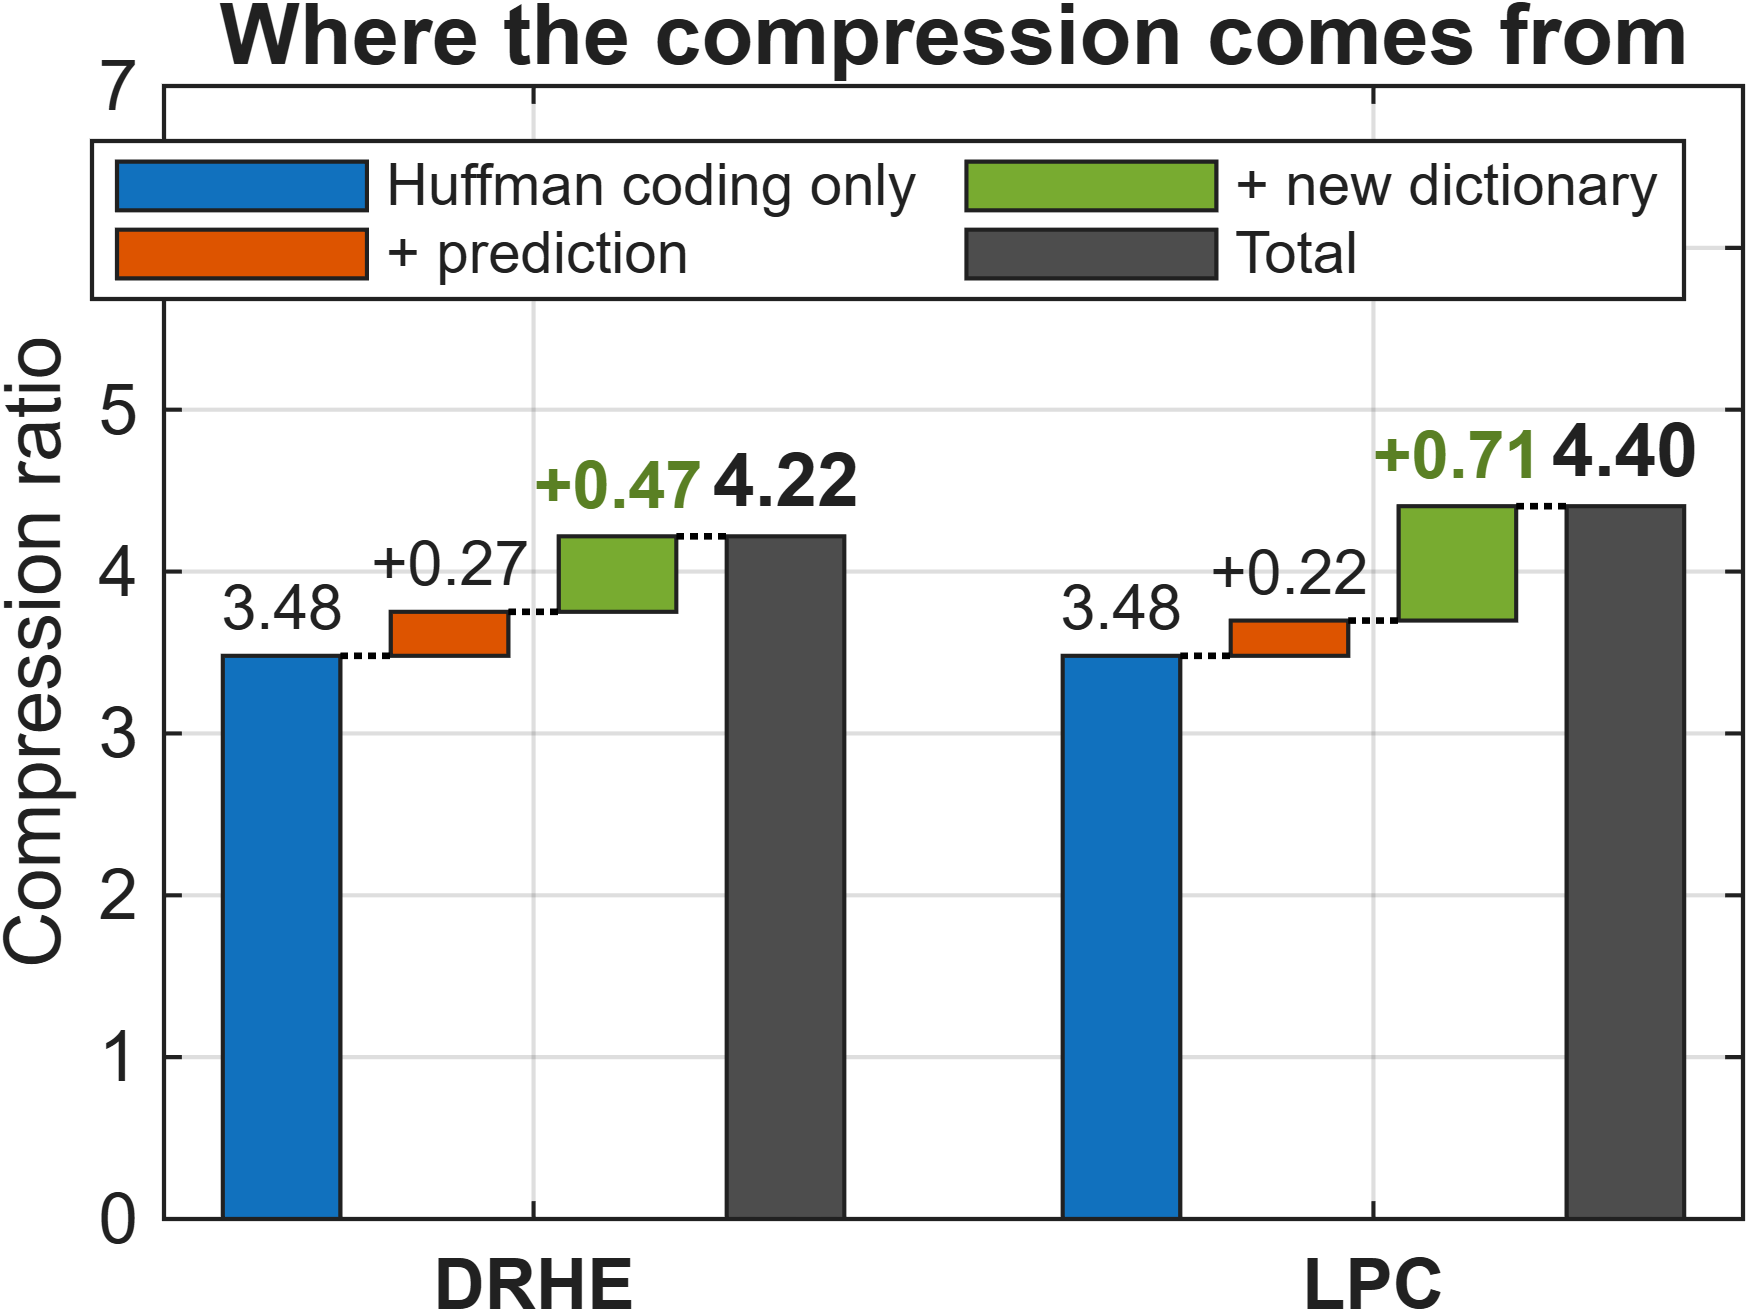
\includegraphics[width=0.62\textwidth]{fig_cr_bars.png}
\caption[Compression ratio, step by step]{The compression ratio built up step by
step. Huffman coding alone reaches \num{3.48}; prediction adds \num{0.22} to
\num{0.27}; the re-derived dictionary adds more than prediction does, for both
algorithms.}
\label{fig:crbars}
\end{figure}

Three things stand out. First, most of the ratio is there before any
prediction: the entropy coder alone achieves \num{3.48}.
Section~\ref{sec:ratiomeaning} explains why --- largely the unused top bits of
the FX16 container, and the sparsity of a range-FFT frame. Second, prediction is
worth a modest but real \SIrange{6}{8}{\percent}. Third, the dictionary adds
more than the predictor does: \num{0.47} for DRHE and \num{0.71} for LPC.

Figure~\ref{fig:residual} shows why prediction helps in the currency the coder
charges in. The share of values that need zero, one or two bits rises, and the
share that need three or more falls; the expensive tail almost disappears.

\begin{figure}[htbp]
\centering
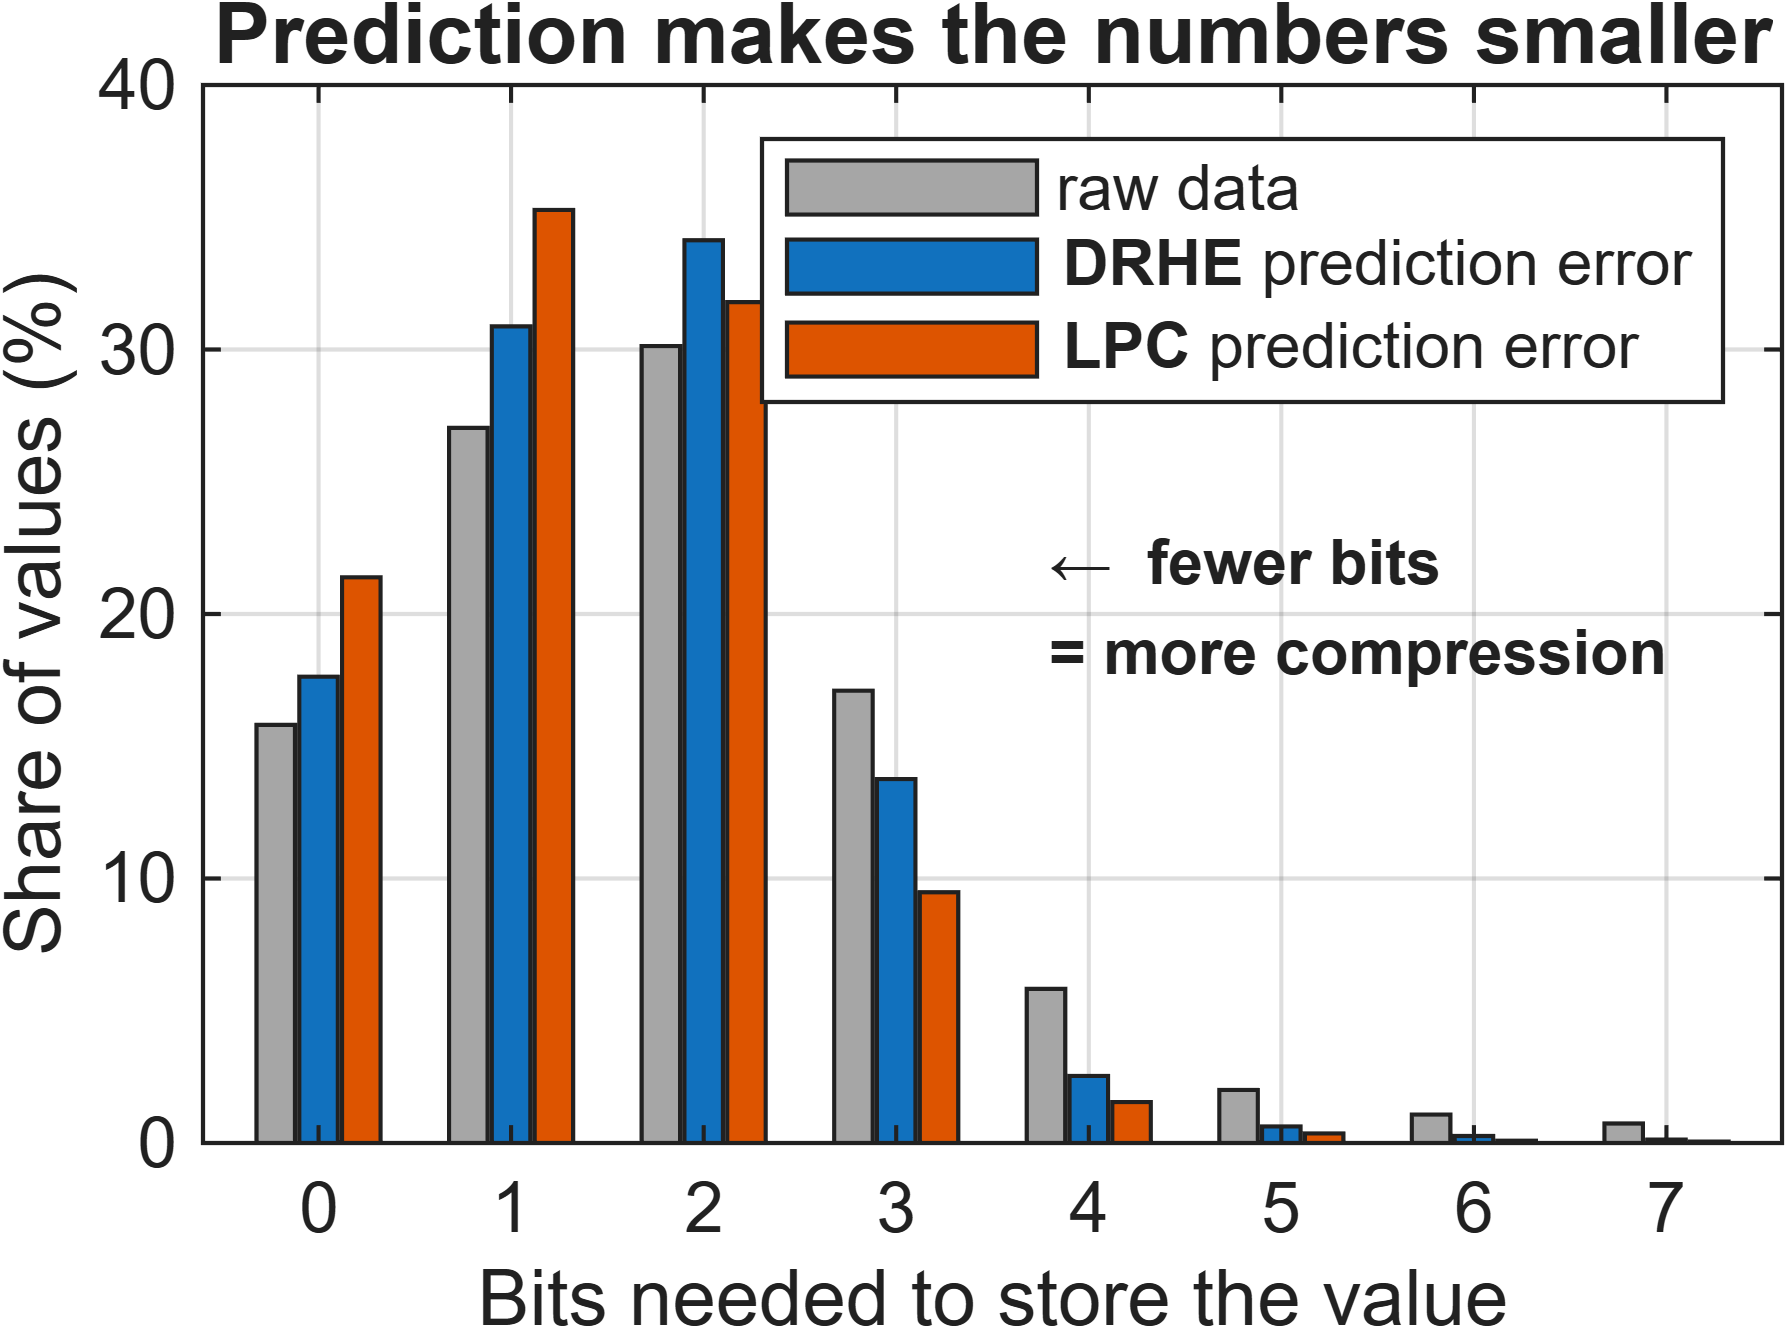
\includegraphics[width=0.62\textwidth]{fig_residual.png}
\caption[Bits needed per value]{How many bits each value needs ($S_4$), for the
raw FX16 codes and for the two algorithms' prediction errors. Prediction moves
values towards the cheap end; most prediction errors need two bits or fewer.}
\label{fig:residual}
\end{figure}

% -------------------------------------------------------------------
\section{The re-derived dictionary}
\label{sec:dictresult}

Table~\ref{tab:dictshare} sets the share of DRHE's prediction errors in each
size category beside the codeword length each dictionary gives it. The original
dictionary gives its shortest codes to categories 2 to 4; on this data most
errors fall in categories 0 to 2, and categories 3 and 4 hold only
\SI{16}{\percent}. The re-derived dictionary gives the three commonest
categories codes of three, two and one bits, and the average codeword falls
from \num{2.70} to \num{2.24} bits per value (from \num{2.80} to \num{2.12} for
LPC).

\begin{table}[htbp]
\centering
\caption[What the re-derived dictionary changes]{Share of DRHE's prediction
errors by size $S_4$, and the codeword length each dictionary assigns
(50 frames, four receive channels). Bold marks the three commonest sizes.}
\label{tab:dictshare}
\small
\begin{tabular}{@{}lrrrrrrr@{}}
\toprule
Size $S_4$ & 0 & 1 & 2 & 3 & 4 & 5 & Average code\\
\midrule
Share of errors (\%)      & \textbf{17.6} & \textbf{30.9} & \textbf{34.1} & 13.8 & 2.5 & 0.6 & ---\\
Code length, original     & 4 & 3 & 2 & 2 & 2 & 5 & \num{2.70} bits\\
Code length, re-derived   & \textbf{3} & \textbf{2} & \textbf{1} & 4 & 5 & 6 & \textbf{\num{2.24} bits}\\
\bottomrule
\end{tabular}
\end{table}

The dictionaries were trained on frames 0--4, so their real test is the 45
frames they did not see. On frames 5--49 DRHE reaches \num{4.207} and LPC
\num{4.372} (Table~\ref{tab:decomp}), within \SI{1}{\percent} of their
all-frame figures: five frames of a scene are enough to fix a dictionary for
the rest of the recording. The C-simulation of the FPGA cores with the
re-derived tables gives \num{4.21704} and \num{4.40345} per frame, matching
MATLAB, and reconstructs all 50 frames exactly.

The dictionary also reverses the ranking of the two algorithms. With the
original dictionary DRHE leads by \SI{1.5}{\percent}; with dictionaries matched
to each algorithm's own errors LPC leads by \SI{4.4}{\percent}. LPC's errors
were always the smaller of the two --- over five frames, \num{4.10} against
\num{4.24} bits per value with the original dictionary, before LPC's \num{0.17}
bits per value of coefficients --- but a dictionary that cannot code anything in fewer than four
bits hides most of that difference.

\subsection{How close to the limit}
\label{sec:coderlimit}

The order-0 entropy of Equation~\eqref{eq:entropy} gives the floor for any code
that treats values independently, and an \emph{ideal} $S_4$ dictionary --- a
Huffman code built on each design's own category counts --- shows how much of the
gap to that floor is the dictionary and how much the $S_4$ construction itself.
Table~\ref{tab:coderlimit} gives both, in bits per value, over five frames.

\begin{table}[htbp]
\centering
\caption[How close the coder gets to the entropy]{Bits per value of the
residuals (coefficient table excluded), five frames, four receive channels:
with the original dictionary, with an ideal $S_4$ dictionary, and the order-0
entropy of the values.}
\label{tab:coderlimit}
\small
\begin{tabular}{@{}lrrrr@{}}
\toprule
Residuals & Original dictionary & Ideal $S_4$ & Entropy & Overhead of original\\
\midrule
No prediction (raw FX16 codes)   & 4.586 & 4.214 & 4.094 & \SI{12.0}{\percent}\\
DRHE, lag $\nTx$                 & 4.240 & 3.711 & 3.516 & \SI{20.6}{\percent}\\
LPC, lags $\nTx$, $2\nTx$        & 4.102 & 3.242 & 3.040 & \SI{34.9}{\percent}\\
\bottomrule
\end{tabular}
\end{table}

\noindent
Two things follow. The $S_4$ construction itself is efficient: the ideal
dictionary comes within 2 to \SI{7}{\percent} of the entropy, so splitting each
value into a coded size and raw payload bits loses little. Almost all of the
original dictionary's excess is the dictionary, and it grows as prediction
improves --- from \SI{12}{\percent} on the raw codes to \SI{35}{\percent} on
LPC's errors --- because the better the predictor, the further its errors sit
below the sizes the original dictionary favours. That is why re-deriving the
dictionary gains more for LPC than for DRHE, and why the gain grows with
prediction quality rather than shrinking.

% -------------------------------------------------------------------
\section{Frame-to-frame variation}
\label{sec:perframe}

\begin{figure}[htbp]
\centering
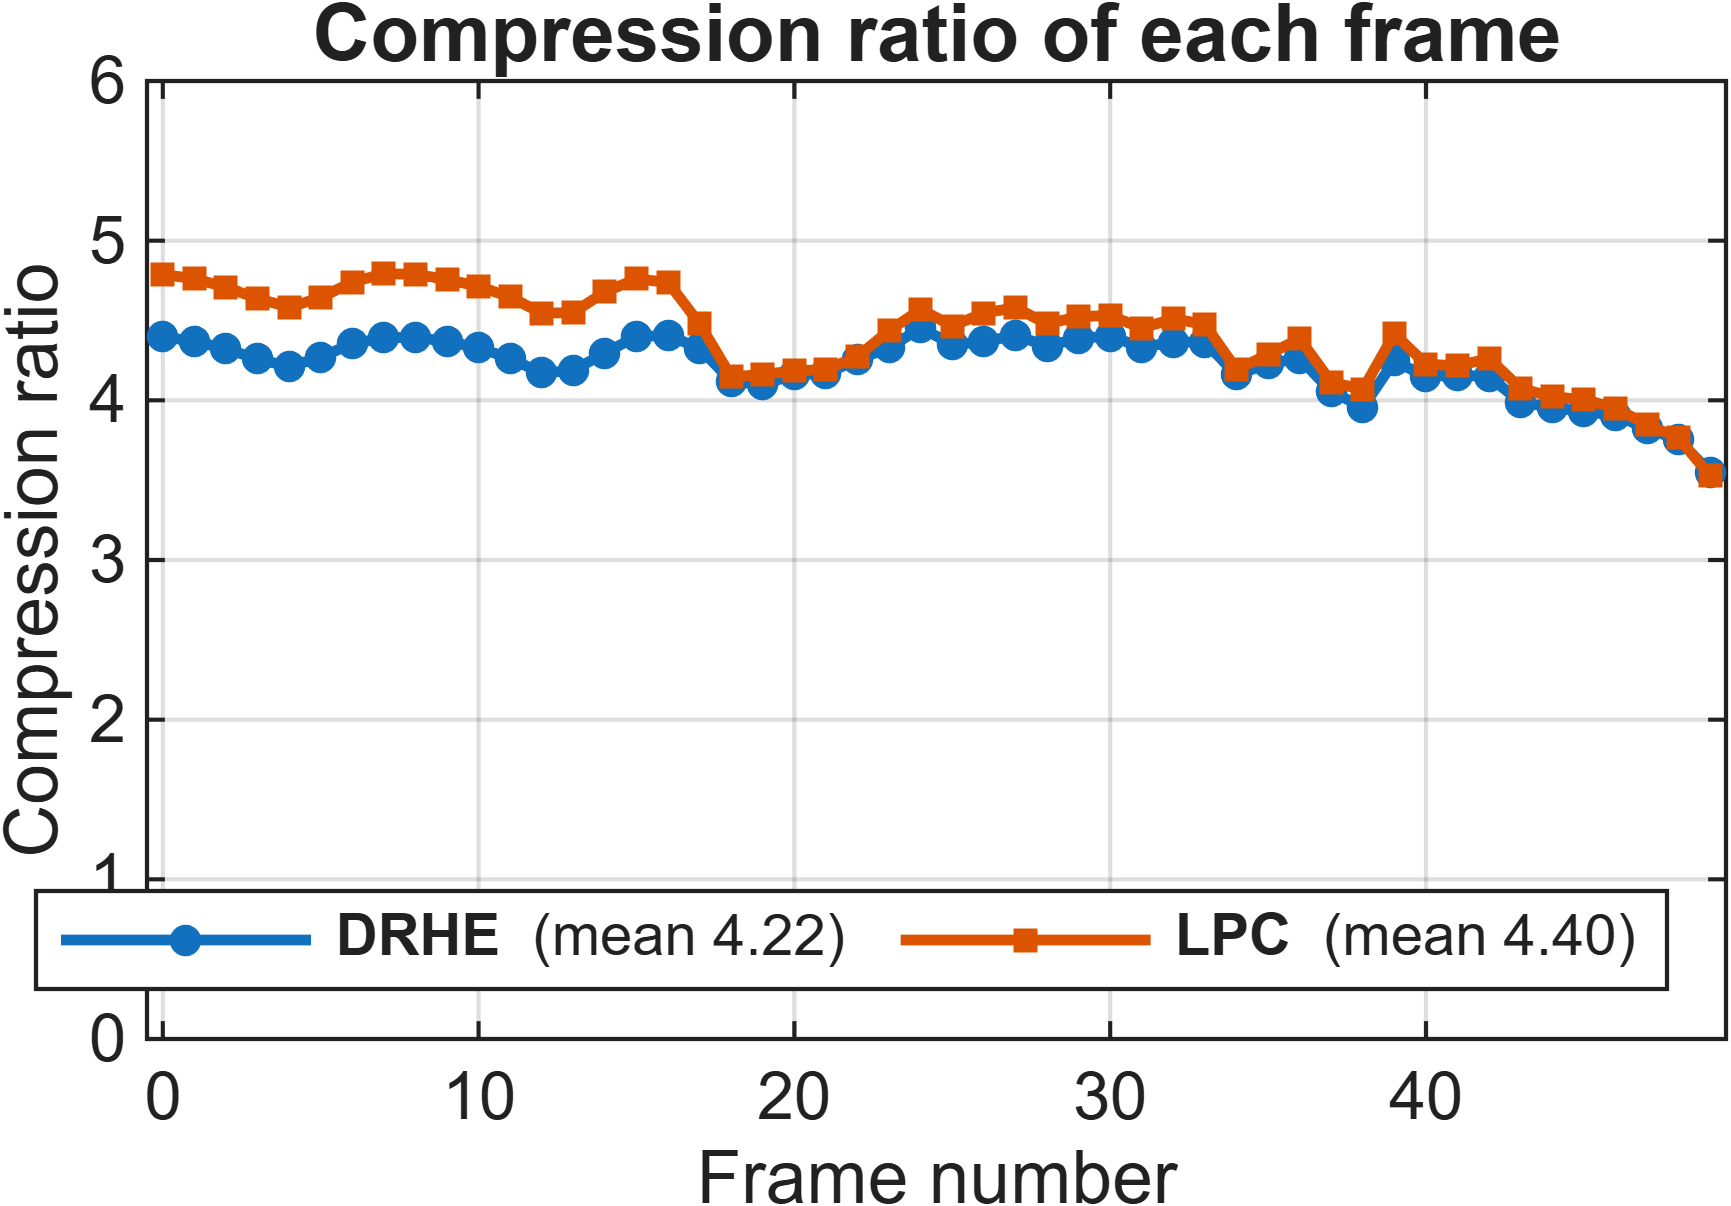
\includegraphics[width=0.62\textwidth]{fig_cr_frames.png}
\caption[Compression ratio of each frame]{Compression ratio of each of the 50
frames, re-derived dictionaries. LPC is ahead on almost every frame; both vary
with the scene in the same way.}
\label{fig:crframes}
\end{figure}

Figure~\ref{fig:crframes} shows the ratio of every frame. It varies by about a
third across the recording, from about \num{3.5} to \num{4.8}, and
the two algorithms move together. The variation tracks how much the scene
contains: frames with more strong returns have larger prediction errors and
compress less, so the per-frame ratio follows the scene rather than any
property of the algorithms. For a system that must carry every frame, it is the
worst frame, not the mean, that sizes the link; at \num{3.5} it still leaves a
wide margin over the \num{2.4}--\num{2.7} required.

% -------------------------------------------------------------------
\section{Verification}
\label{sec:verifres}

Every level of the ladder of Section~\ref{sec:ladder} that has been run
passed with $\mathrm{MaxDiff} = 0$:

\begin{itemize}
\item \textbf{C-simulation}, 50 frames (\num{4915200} complex samples,
\num{157286400} input bits per design): both compressors, with both the
original and the re-derived dictionaries, reconstruct every sample exactly. The
bit counts agree with MATLAB on every frame once the zero padding of the last
256-bit output word is counted: MATLAB's LPC model includes it and agrees
exactly, and its DRHE model omits it, so the hardware's DRHE counts exceed
MATLAB's by 15 to 252 bits, always less than one word.
\item \textbf{RTL co-simulation}: both compressors reconstruct exactly.
\item \textbf{Edge cases}: all eight synthetic cases of
Table~\ref{tab:edgecases} pass for both algorithms. Uniformly random input
\emph{expands} by \SI{67}{\percent} (CR \num{0.60}), as any lossless coder must
on incompressible data: every value lands in a high category, costing a long
codeword plus up to 15 payload bits.
\item \textbf{Board}: with the original dictionary, both compressors produced
compressed output \emph{byte-identical} to the C-simulation on all 50 frames,
and every frame, decompressed on the PC, matched the input exactly. Mean compression ratio on the
board was \num{3.7508} for DRHE (range \numrange{3.517}{3.815}) and
\num{3.6968} for LPC (\numrange{3.461}{3.761}), exactly the C-simulation
figures. The bitstreams with the re-derived dictionaries differ only in the
contents of the codeword table and were C-simulated lossless on all 50 frames;
\pending{board run of the re-derived-dictionary bitstreams}.
\item \textbf{On-chip decompression}: the \texttt{\_full} bitstreams, with the
decompressor on the FPGA, build and meet timing (Table~\ref{tab:builds}); the
decompressors were verified lossless on all 50 frames in C-simulation and on
the PC with the board's compressed output. \pending{board run of the
on-chip decompression builds}.
\end{itemize}

\noindent
Agreement at the board level is the strongest result here: the bytes produced
by the FPGA are the bytes the simulation predicted. The original-dictionary
ratios are therefore measured hardware figures, and since the re-derived builds
change only the contents of one table, their C-simulated ratios are what the
same hardware will produce.

% -------------------------------------------------------------------
\section{Speed and latency on the board}
\label{sec:boardtiming}

Table~\ref{tab:timing} gives the timing measured on the board over 50 frames,
and Figure~\ref{fig:timing} draws it.

\begin{table}[htbp]
\centering
\caption[Measured timing on the board]{Timing measured on the KCU116 at
\SI{100}{\mega\hertz}, 50 frames of \SI{393216}{\byte}. Latency is from the last
input word read to the last output word written (Section~\ref{sec:metrics}).}
\label{tab:timing}
\small
\begin{tabular}{@{}lrr@{}}
\toprule
& \textbf{DRHE} & \textbf{LPC}\\
\midrule
Clock cycles per frame          & \num{61472}   & \num{325366}\\
Time per frame                  & \textbf{\SI{0.61}{\milli\second}} & \SI{3.25}{\milli\second}\\
Frames per second               & \num{1627}    & \num{307}\\
Input throughput                & \textbf{\SI{5.12}{Gbit/s}} & \SI{0.97}{Gbit/s}\\
End-to-end latency              & \textbf{\SI{13.1}{\micro\second}} & \SI{3006}{\micro\second}\\
\quad as a share of the frame time & \SI{2}{\percent} & \SI{92}{\percent}\\
Decompression time per frame    & \pending{\texttt{\_full} run} & \pending{\texttt{\_full} run}\\
\bottomrule
\end{tabular}
\end{table}

\begin{figure}[htbp]
\centering
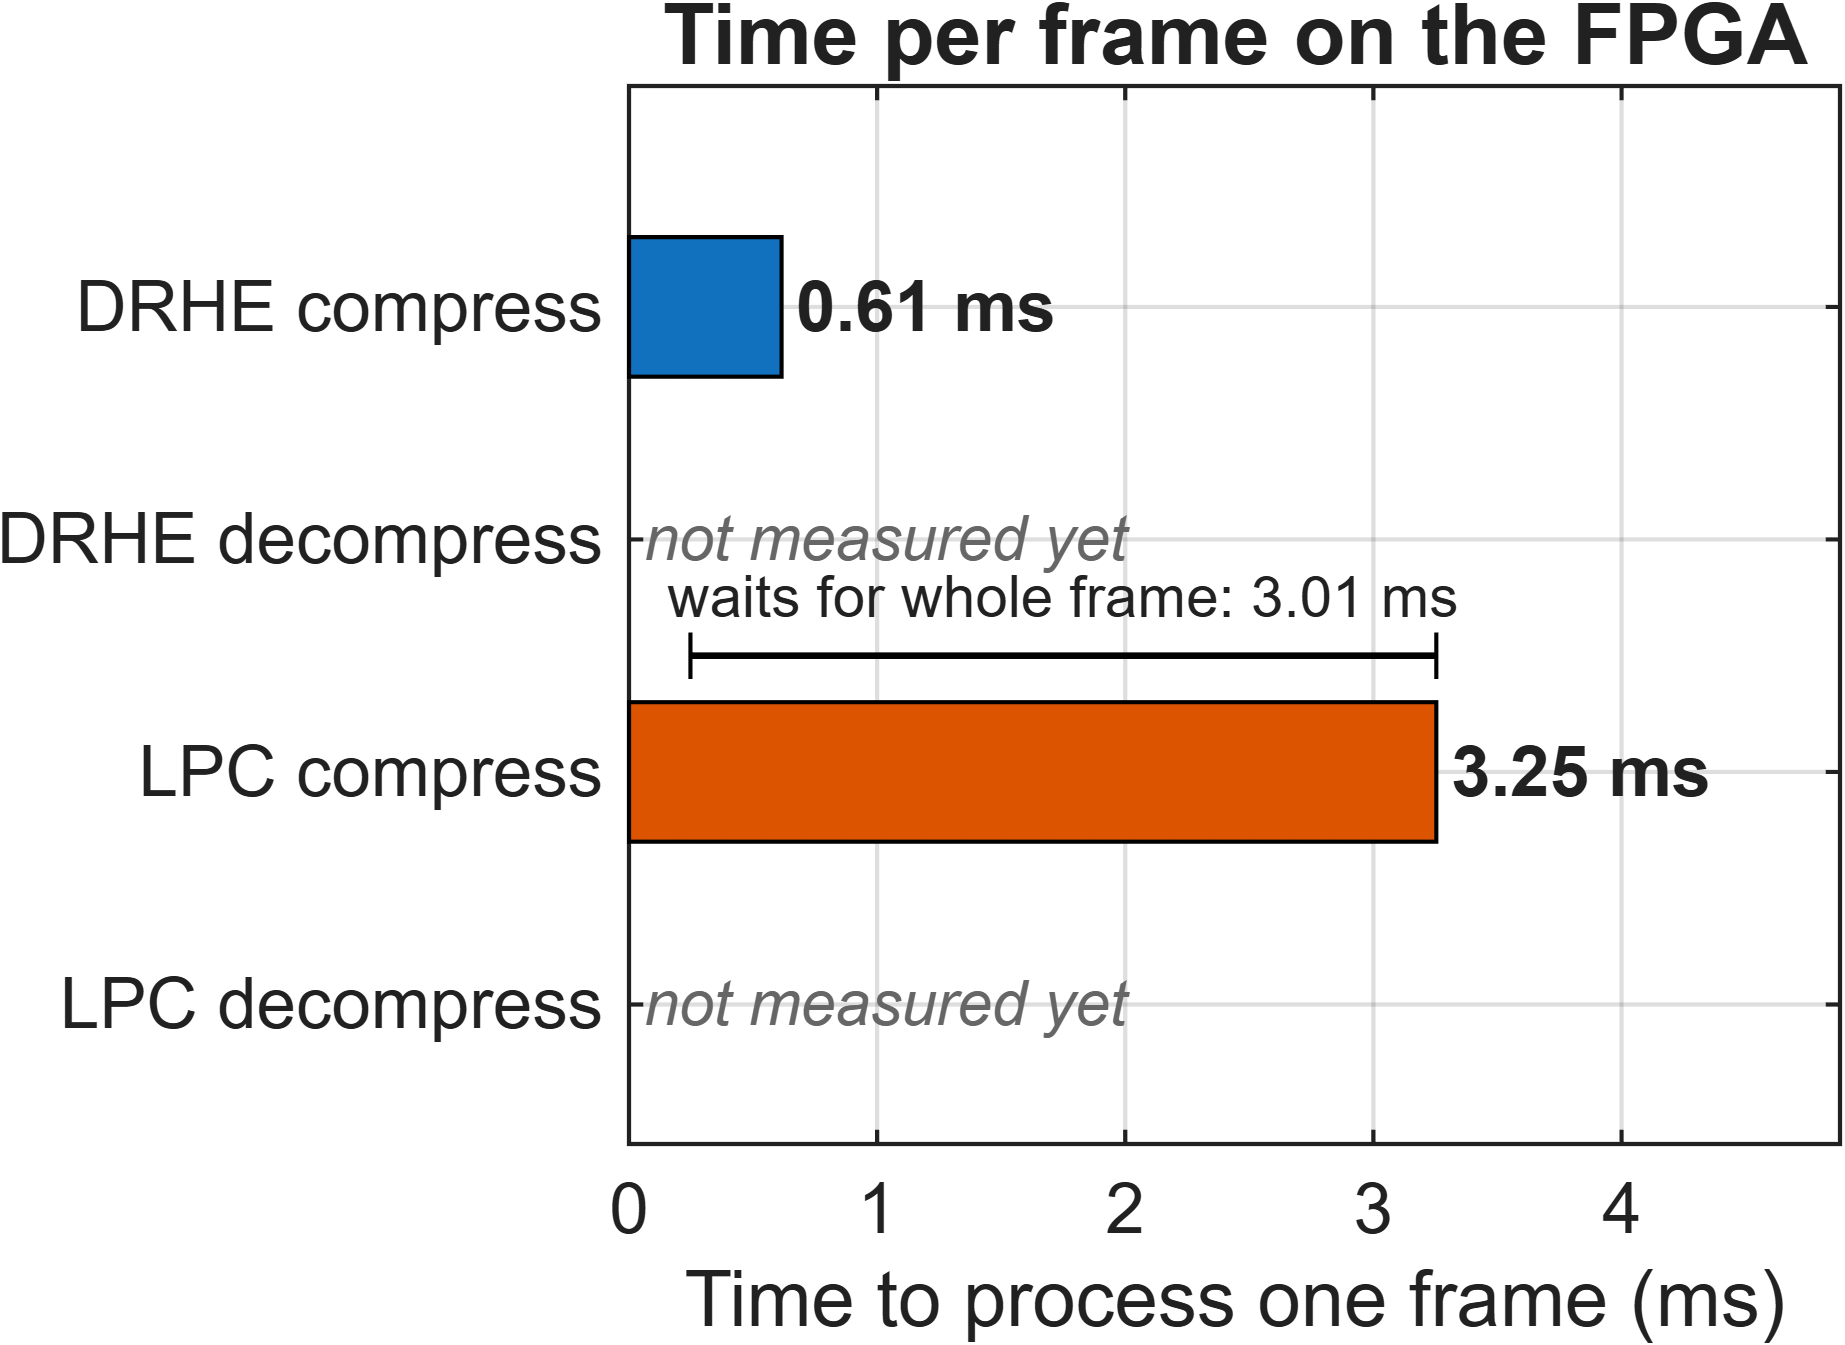
\includegraphics[width=0.62\textwidth]{fig_timing.png}
\caption[Time per frame on the FPGA]{Time to process one frame on the FPGA. DRHE
outputs as the data arrives; LPC must wait for the whole frame (bracket) before
it can output anything.}
\label{fig:timing}
\end{figure}

\paragraph{DRHE streams.} Its time per frame, \SI{0.61}{\milli\second}, is two
clocks per input beat ($\mathrm{II} = 2$) plus a short pipeline fill on each
ramp. Its latency is \SI{13.1}{\micro\second}: the last compressed word leaves
almost as soon as the last raw word arrives. The core's own pipeline accounts
for about a microsecond of that; the rest is most likely data still in flight in
the DMA and interconnect when the last input word is read, though this was not
measured separately.

\paragraph{LPC waits.} Its time per frame is \SI{3.25}{\milli\second}, 5.3 times
DRHE's, and \SI{92}{\percent} of it --- \SI{3.0}{\milli\second} --- comes
\emph{after} the last input word has arrived, because the coefficients cannot be
computed until every ramp of the frame is in. That is 230 times DRHE's latency.
It is not an implementation weakness that better scheduling would remove: as
long as the coefficients are fitted to the frame being compressed, the first
output bit has to wait for the last input sample.

Both are fast in absolute terms. The ColoRadar cascade records at
\SI{5}{\hertz}, a frame every \SI{200}{\milli\second}, so DRHE uses
\SI{0.3}{\percent} of the frame period and LPC under \SI{2}{\percent}. Section~\ref{sec:scaling} considers what happens
on larger frames.

% -------------------------------------------------------------------
\section{Chip resources}
\label{sec:resources}

Table~\ref{tab:resources} gives the post-route resources of each core, taken
from the hierarchical utilisation report of the \texttt{\_full} builds, and
Figure~\ref{fig:resources} draws them as a share of the chip.

\begin{table}[htbp]
\centering
\caption[Resources per core]{Post-route resources of each core on the
\texttt{XCKU5P} (\num{216960} LUT, \num{433920} FF, 480 BRAM, \num{1824} DSP).
BRAM is in 36\,Kb blocks.}
\label{tab:resources}
\small
\begin{tabular}{@{}llrrrr@{}}
\toprule
& & LUT & FF & BRAM & DSP\\
\midrule
DRHE & compressor   & \num{35444} & \num{23528} & 40   & 132\\
     & decompressor & \num{14155} & \num{9245}  & 32.5 & 46\\
     & \textbf{both} & \textbf{\num{49599}} (\SI{23}{\percent}) & \num{32773} & 72.5 & 178\\
\midrule
LPC  & compressor   & \num{33738} & \num{20165} & 98   & 158\\
     & decompressor & \num{20034} & \num{8371}  & 0    & 8\\
     & \textbf{both} & \textbf{\num{53772}} (\SI{25}{\percent}) & \num{28536} & 98 & 166\\
\bottomrule
\end{tabular}
\end{table}

\begin{figure}[htbp]
\centering
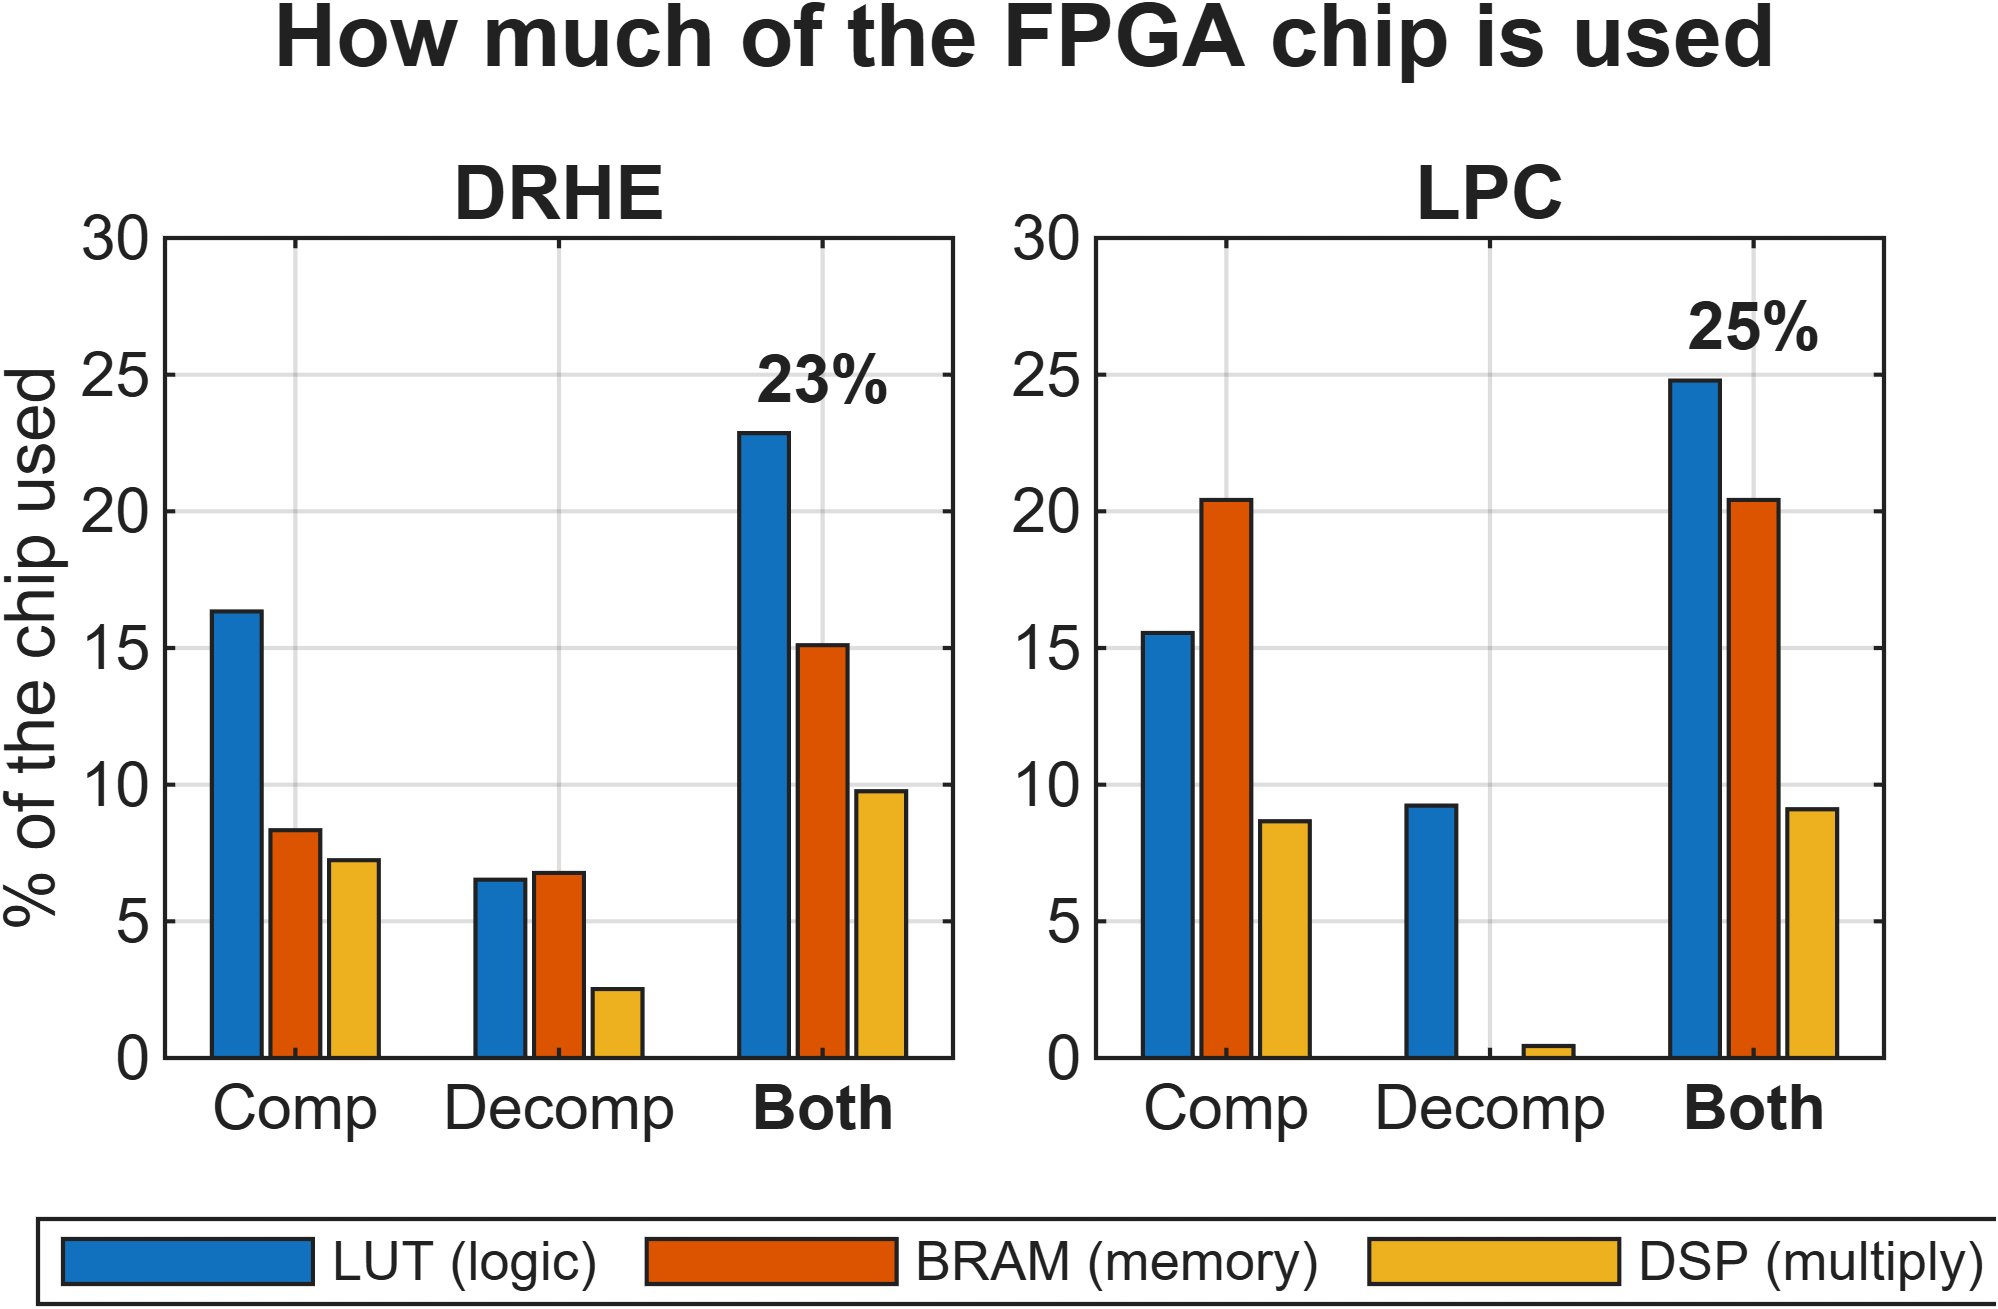
\includegraphics[width=0.66\textwidth]{fig_resources.png}
\caption[FPGA resources]{Share of the chip used by each core, for the
compressor, the decompressor, and both together.}
\label{fig:resources}
\end{figure}

Encoder and decoder together use under a quarter of the chip's logic for both
algorithms, and the whole test system --- processor, memory controller, DMAs and
both cores --- uses \SI{38}{\percent} (DRHE) and \SI{40}{\percent} (LPC)
(Table~\ref{tab:builds}). The two compressors cost almost the same logic. They
differ in memory: LPC's compressor needs 98 block RAMs, most of them its frame
buffer, against DRHE's 40 for predictor state. The decoders invert this. The
DRHE decoder carries its own floating-point predictor and its state, while the
LPC decoder needs no data memory at all and only eight DSP slices, because the
coefficients arrive ready-made in the bitstream.

% -------------------------------------------------------------------
\section{The two algorithms side by side}
\label{sec:headtohead}

\begin{table}[htbp]
\centering
\caption[DRHE and LPC compared]{DRHE and LPC compared on every measured
quantity. Bold marks the better of the two on each row.}
\label{tab:headtohead}
\small
\begin{tabular}{@{}lrr@{}}
\toprule
& \textbf{DRHE} & \textbf{LPC}\\
\midrule
Lossless (C-sim, 50 frames; board, original dictionary) & yes & yes\\
Compression ratio, original dictionary (board)    & \textbf{\num{3.75}} & \num{3.70}\\
Compression ratio, re-derived dictionary (C-sim)  & \num{4.22} & \textbf{\num{4.40}}\\
Time per frame                                   & \textbf{\SI{0.61}{\milli\second}} & \SI{3.25}{\milli\second}\\
End-to-end latency                               & \textbf{\SI{13.1}{\micro\second}} & \SI{3006}{\micro\second}\\
First output available                           & \textbf{immediately} & after the whole frame\\
Compressor frame buffer                          & \textbf{none} & \SI{3.0}{\mebi bit}\\
Encoder + decoder LUTs                           & \textbf{\SI{23}{\percent}} & \SI{25}{\percent}\\
Encoder + decoder BRAM (36\,Kb blocks)          & \textbf{72.5} & 98\\
Side information                                 & \textbf{none} & \SI{1.04}{\percent}\\
\bottomrule
\end{tabular}
\end{table}

Table~\ref{tab:headtohead} collects the results. On compression ratio the two
are close, and which one leads depends on the dictionary: DRHE by
\SI{1.5}{\percent} with the original one, LPC by \SI{4.4}{\percent} with
dictionaries matched to each. On logic they are level. On time, latency and
memory DRHE is clearly ahead: it compresses a frame five times faster, needs no
frame buffer, and its output lags its input by microseconds rather than
milliseconds. Chapter~\ref{ch:discussion} weighs these against each other.
